\section{\textsc{IntraCFG}: Intraprocedural Framework for Source-Level Control-Flow Analysis}%
\label{sec:IntraCFG}
The techniques of CFG construction have seen significant advancements
in recent years, with various frameworks being proposed to aid in the construction
of precise intraprocedural CFGs~\cite{smits2020flowspec,10.1016/j.scico.2012.02.002}.
We contribute to the state-of-the-art by introducing \textsc{IntraCFG}, a declarative, RAG-based,
and language-independent framework for constructing precise intraprocedural CFGs.
In this section we give an overview of \textsc{IntraCFG}, and more details are available
in Paper~\ref{paper:intraj}.

Unlike most other frameworks, which build CFGs on the IR level,
e.g.,  bytecode, \textsc{IntraCFG}'s approach superimposes the CFGs
on the AST. This allows for accurate client analysis,
as the CFGs are constructed directly on the source code level rather than an
intermediate representation.
Diffrently from the existing RAG-based framework~\cite{10.1016/j.scico.2012.02.002},
\textsc{IntraCFG} enables the construction of \textsc{AST-Unrestricted} CFGs,
which are CFGs whose shape is not restricted to the AST structure.
\subsection{Overall Architecture}
The overall architecture of how to use our proposed framework, \textsc{IntraCFG}, is shown in Figure~\ref{fig:intraCFG}.
\textsc{IntraCFG} provides the skeleton and default behaviour for constructing CFGs,
which can be instantiated for specific languages\footnote{\textbf{\texttt{IntraX}} in the diagram.}, e.g., Java or Teal.
The \emph{Control-flow analysis} (CFA) module is specifically tailored for a particular 
programming language and implements the interfaces defined in \textsc{IntraCFG}.
This module is responsible for constructing the CFG for the program. 
Once the CFA module has generated the CFG, 
other client analyses can added, for example, different dataflow analyses.
The compiler module plays a crucial role as it defines the AST nodes
on which the CFA module heavily relies. The compiler also provides access to 
several APIs that can be used by the CFA module and client analyses, such as 
the type of a variable or the constant value of an expression, to perform 
advanced optimizations.

\begin{figure}[H]
    \centering
    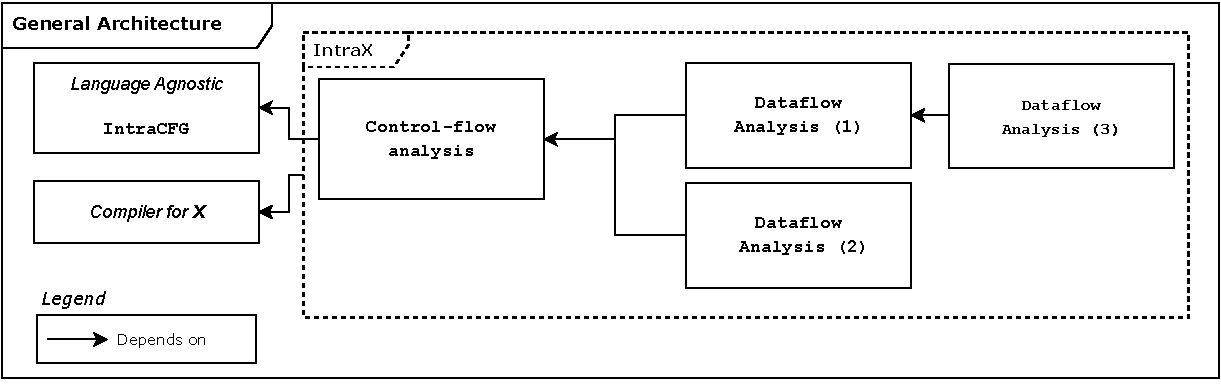
\includegraphics[width=1\textwidth]{kappa/img/architecture.pdf}
    \caption{\label{fig:intraCFG} Overall architecture of instantiating \textsc{IntraCFG} for a language \textbf{X}.}
\end{figure}

\textsc{IntraCFG} consists of several key components, including interfaces, attribute equations that define the
default behaviour, and APIs. The interfaces provide the structure for the
CFG, and the attribute equations define the default behaviour for the CFG
construction. 
In the language dependent control-flow module, implementations of the \textsc{IntraCFG}
interfaces are added to the AST types of the language. This can be done according to the
precision desired for the CFG.
% Language specific AST nodes implement the different interfaces
% according to the precision desired for the CFG.

\textsc{IntraCFG} has APIs in the form of attributes, allowing clients to access entry
and exit nodes and to traverse the CFG.
The language-independent nature of \textsc{IntraCFG} allows for easy integration
with various programming languages and enables the construction of precise CFGs
for those languages. The use of attribute equations and interfaces also allows
for a high degree of flexibility in the CFG construction process,
enabling the customization of the CFG to fit the specific needs of the
analysis being performed.

% Additionally, language-specific dataflow analysis, such as \texttt{NullPointerException} or
% \texttt{IndexOutOfBound} detection, can be built on top of the framework.





\subsection{\textsc{IntraJ}: \textsc{IntraCFG} for Java}
\label{sec:IntraJ}
To demonstrate \textsc{IntraCFG} applicability, we developed
\textsc{IntraJ}, an instance of the framework for the Java programming language.
We built \textsc{IntraJ} upon the \textsc{ExtendJ} extensible Java compiler~\cite{DBLP:conf/oopsla/EkmanH07}.
% The complete architecture of \textsc{IntraJ} is shown in Figure~\ref{fig:intraJ}.
\begin{figure}[H]
    \centering
    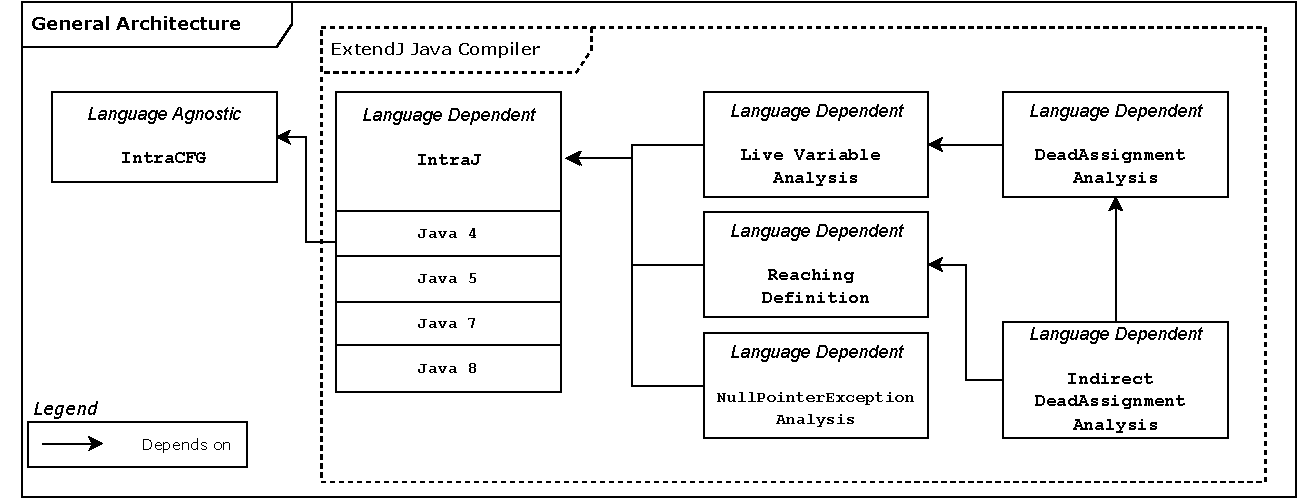
\includegraphics[scale=0.52]{kappa/img/architecturejava.pdf}
    \caption{\label{fig:intraJ} Overall architecture of instansiating \textsc{IntraCFG} for the Java language.}
\end{figure}

%Discussing modularity
As seen in Figure~\ref{fig:intraJ}, we designed \textsc{IntraJ}
following a  modular approach, and we separately
instantiated the framework for different versions of Java, such as Java 4,
Java 5, Java 7 and Java 8.
\textsc{ExtendJ} has a similar modularisation of different Java versions. 
When \textsc{ExtendJ} is extended to support new versions of Java, this approach
will allow us to extend \textsc{IntraJ} in a corresponding way.
This approach allows us and the users of \textsc{IntraJ}
to easily extend the framework to support new versions of Java.

% Discussing precision
The degree of precision in creating CFGs using \textsc{IntraCFG} can differ in order
to meet the requirements of a given application.
This flexibility allows the framework users to optimise the analysis's efficiency 
by selectively excluding/including specific AST nodes from the CFG.
For example, nodes such as \astnode{WhileStmt}, which are essential for the
construction of CFGs, as they are used to define the shape of CFGs, can be excluded
from the CFGs as all relevant execution points for the \astnode{WhileStmt} are
already captured by other AST nodes, i.e., evaluation of the condition, and execution
of the body.
\begin{figure}[H]
	\centering
	\begin{tikzpicture}
		\node (a) at (3.5,0) {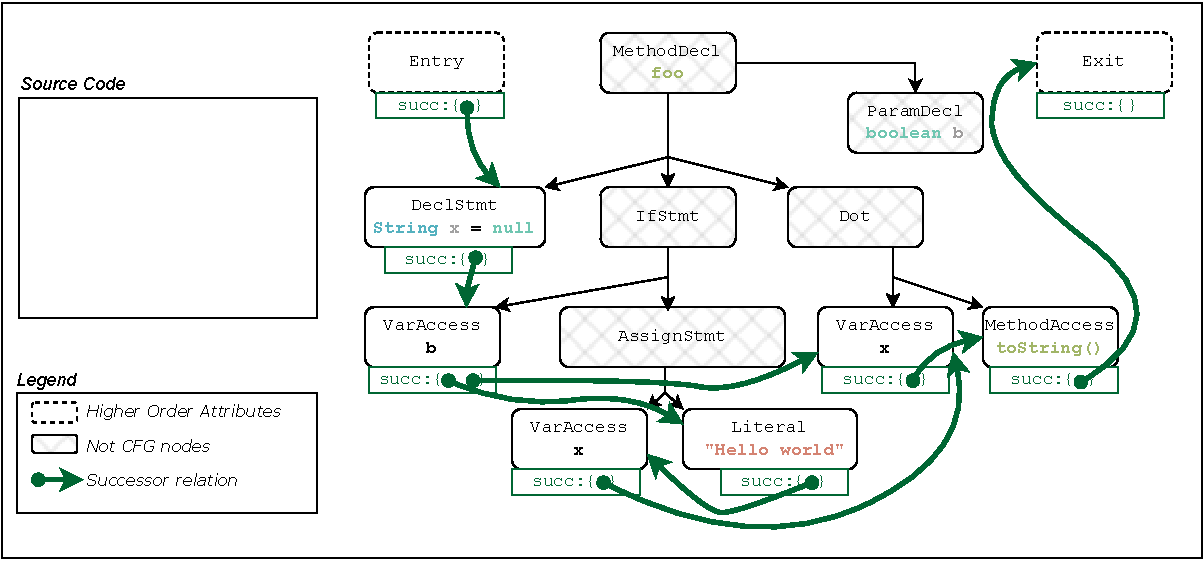
\includegraphics[scale=0.55]{kappa/img/exampleAST.pdf}};
		\node[scale=0.65] (b) at (-0.6,0.7) {
			\begin{lstlisting}[language=JastAdd]
void foo(boolean b){
  String x = null;
  if(b) {
    x = "Hello World";
  }
  x.toString();
}
			\end{lstlisting}
		};
	\end{tikzpicture}
	\caption{\label{fig:CFG} CFG of the \texttt{foo} Java method.}
\end{figure}

The example in Figure~\ref{fig:CFG} is a visual representation of the AST and CFG of the
\texttt{foo} Java method. The figure illustrates the ability of the framework to tailor the CFG
to the specific requirements of the analysis and eliminate unnecessary complexity for improved performance.
In this example, nodes like \astnode{IfStmt} or \astnode{Dot} are not included in the CFG,
resulting in a more concise but precise representation of the control flow of the program.
On the other hand, the precision of the CFGs can be improved by synthesising new nodes and subtrees as HOAs.
For instance, we designed \textsc{IntraJ} to compute an exception-sensitive
control-flow analysis, i.e., new AST subtrees are synthesized for each possible exceptional path.
The resulting CFGs are more precise but also more complex, resulting
in higher memory consumption and a more extended analysis time.



In \textsc{IntraJ}, we implemented five different dataflow analyses:
\begin{itemize}
  \item \emph{Live Variable Analysis}: computes the set of variables that are live at each point in the program.
  \item \emph{Reaching Definition}: computes the set of definitions that reach each point in the program.
  \item \emph{Null Pointer Analysis}: detects possible null pointer dereferences.
  \item \emph{Dead Assignment Analysis}: detects assignments to l-values that are never used from that point on.
  \item \emph{Indirect Dead Assignment Analysis}: detects assignments to l-values which uses always flow to a dead assignment.
\end{itemize}
All the analyses rely on the result of the control-flow analysis. The analyses use
the \Ahoa{CFGRoot}{entry} and \Ahoa{CFGRoot}{exit} attributes of the CFG, as well as the \Asyn{CFGNode}{succ} and \Asyn{CFGNode}{pred}
attributes of each node.
Each analysis is implemented as a separate aspect.
Still, some analyses' results are used as input for other analyses. For instance,
the result of Live Variable Analysis is used as input for the Dead Assignment Analysis.
Similarly, the result of Dead Assignment Analysis is used to compute Indirect Dead Assignment Analysis.

The implemented analyses are instances of the monotone frameworks (see Section~\ref{sec:monotoneframeworks}).
Each analysis defines its abstract domain, transfer function and \emph{in} and
\emph{out}\footnote{Or \emph{kill} and \emph{gen}.} circular attributes for each \astnode{CFGNode} (i.e., \AcircSyn{CFGRoot}{in} and  \AcircSyn{CFGRoot}{out}).
While the core of each dataflow analysis is language independent, relying only on the
attributes defined by \textsc{IntraCFG}, there are language dependencies in the 
transfer function, which is modelled as a circular parametrised attribute.
The transfer function attribute is define for each AST node in the CFG to capture the semantics of passing
through that node, and for different AST node types, the transfer function is defined differently.
For example, in the case of \code{NullPointerException} analysis,
the general and language-independent definition of the transfer function is
defined as follows:
\begin{lstlisting}[language=JastAdd]
  syn CFGNode.trFun(Gamma gamma) circular [new Gamma()] {
    return gamma;
  }
\end{lstlisting}
While the transfer function for \astnode{AssignStmt} is defined as follows:
\begin{lstlisting}[language=JastAdd]
  eq AssignStmt.trFun(Gamma gamma) {
    Variable decl = getDeclarationLHS();
    if (getNullyRHS()){
      gamma.put(decl, NULL);
    }
    else{
      gamma.put(decl, NOTNULL);
    }
    return gamma;
  }
\end{lstlisting}


\subsubsection{\textsc{IntraJ} Artifact Evaluation}
Artifact evaluation is an essential part of the scientific process as it enables
researchers to demonstrate the reproducibility and practicality of their work~\cite{KrishnamurthiArtifact2013}.
It also allows other researchers to build upon and reuse the work in their
studies, helping to advance the field as a whole.

In this context, our artifact, \textsc{IntraJ}, was presented at the
ROSE\footnote{\textbf{R}ecognizing and Rewarding \textbf{O}pen Science in \textbf{SE},
\url{https://icsme2021.github.io/cfp/AEandROSETrack.html}} Festival 2021,
co-located with ICSME2021 and SCAM2021. The artifact was awarded the \emph{Open Research Objects}
(ORO) and \emph{Research Objects Reviewed} (ROR) badges.
The ORO badge indicates that the artifact is publicly accessible and has been
\emph{``placed in an archival repository, with a unique identifier and a link provided''}.
The ROR badge highlights that the artifact has been
\emph{``very carefully documented and structured, making it suitable for reuse and repurposing
in accordance with research community norms and standards''.} This recognition
demonstrates the high quality and usefulness of the artifact.

\begin{figure}[H]
  \centering
  \begin{subfigure}{0.3\linewidth}
    \includegraphics[width=\linewidth]{kappa/img/Open_research.png}
    \caption{Open Research Objects (ORO) badge}
    \label{fig:ORO}
  \end{subfigure}\hspace{2cm}
  \begin{subfigure}{0.3\linewidth}
    
\includegraphics[width=\linewidth]{kappa/img/Research_Objects.png}
    \caption{Research Objects Reviewed (ROR) badge}
    \label{fig:ROR}
  \end{subfigure}
  \caption{Badges awarded to the artifact.}
  \label{fig:badges}
\end{figure}


\section{\textsc{IntraTeal}: \textsc{IntraCFG} for TEAL}
\label{sec:intraTeal}
As a further demonstration\footnote{This application of \textsc{IntraCFG} has not been
peer-reviewed by the scientific community.} of the applicability of \textsc{IntraCFG},
we developed \textsc{IntraTeal}, an implementation of \textsc{IntraCFG} for the Teal programming language.
% \subsection{The TEAL Programming Language}
% \label{sec:teal}
TEAL v0.4 (Typed Easily Analysable Language) is a programming language designed by Christoph Reichenbach and used in the
program analysis\footnote{\url{https://fileadmin.cs.lth.se/cs/Education/EDAP15/2022/web/index.html}} course at Lund University.
TEAL aims to provide a language that allows students to
focus on the challenges of performing program analysis on a real-world language
without being overwhelmed by the details of a fully-featured language.
% One of the key features of TEAL is that it is an object-oriented language,
% which means that it allows the creation of classes and objects that can inherit
% characteristics and behaviour from one another. However, it does not have a dynamic
% dispatcher, which means that the method that is called for an object at run-time
% is determined at compile-time based on the type of the object.
TEAL is divided in layers, with each version building
upon the features of the previous one. TEAL-0 is the most basic version and includes
support for variable declarations and use, procedures, and basic control structures such as if
and while statements. TEAL-1 introduces the enhanced-for loop, and TEAL-2
introduces user-defined classes. 
In this section,  we will use TEAL-0 to exemplify the use of RAGs
and \textsc{IntraCFG}.
The concrete and abstract grammar of TEAL-0 are shown in Figure~\ref{fig:tealGrammar}.
The concrete grammar is used for parssing. The abstract grammar is given using
\textsc{JastAdd} syntax, and will be used in examples throughout this section 
to describe analyses in TEAL.
\newsavebox{\mylistingbox}

\begin{figure}[H]
    \hspace*{-1cm}
    \begin{minipage}{0.5\textwidth}
        \[\footnotesize
        \begin{array}[t]{lcl@{\hspace{0.4cm}}}
          \nta{Program} & \Prod & \ntstar{Decl} \\
          \\
          \nta{Decl} & \Prod & \nt{VarDecl}\ \\
                       & \VB & \vterminal{fun}\ \terminal{id}\ \vterminal{(}\ \ntq{formals}\ \vterminal{)}\\
                       &&  \nt{optTyped}\ \vterminal{=}\ \nt{stmt} \\
          \\
          \nta{VarDecl} & \Prod & \vterminal{var}\ \terminal{id}\ \nt{optTyped} \\
                        & \VB   & \vterminal{var}\ \terminal{id}\ \nt{optTyped}\ \vterminal{:=}\ \nt{Expr} \vterminal{;}\\
          \\
          \nta{formals} & \Prod & \terminal{id}\ \nt{optTyped} \\
                        & \VB & \terminal{id}\ \nt{optTyped}\ \vterminal{,}\ \nt{formals}\\
                      \\
          \nta{optTyped} & \Prod & \vterminal{:}\ \nt{Type}\\
                        & \VB{} & \varepsilon \\
          \\
          \nta{Type} & \Prod & \Cty{int}\ \VB\ \Cty{string}\ \VB\ \Cty{any} \\
                     & \VB   & \Cty{array}\ \Cty{[}\ \nt{Type}\ \Cty{]} \\
          \\
          \nta{Block} & \Prod & \vterminal{\{}\ \ntstar{Stmt}\ \vterminal{\}} \\
          \\
          \nta{Expr} & \Prod & \nt{Expr}\ \nt{binop}\ \nt{Expr} \\
                     & \VB   & \vterminal{not}\ \nt{Expr} \\
                     & \VB   & \vterminal{(}\ \nt{Expr}\ \nt{optTyped}\ \vterminal{)} \\
                     & \VB   & \nt{Expr}\ \vterminal{[}\ \nt{Expr}\ \vterminal{]} \\
                     & \VB   & \terminal{id}\ \vterminal{(}\ \ntq{actuals}\ \vterminal{)} \\
                     & \VB   & \vterminal{[}\ \ntq{actuals}\ \vterminal{]} \\
                     & \VB   & \vterminal{new}\ \nt{Type}\ \vterminal{(}\ \nt{Expr}\ \vterminal{)} \\
                     & \VB   & \terminal{int}\ \VB\ \terminal{string}\ \VB\ \vterminal{null} \\
                     & \VB   & \terminal{id} \\
          \\
          \nta{actuals} & \Prod & \nt{Expr} \\
                        & \VB   & \nt{Expr} \vterminal{,}\ \nt{actuals} \\
          \\
          \nta{binop} & \Prod &
              \vterminal{+}
                      \ \VB\ \vterminal{-}
                      \ \VB\ \vterminal{*}
                      \ \VB\ \vterminal{/}
                      \ \VB\ \vterminal{\%}\\
                      & \VB& \vterminal{==}
                      \ \VB\ \vterminal{!=}\\
                      & \VB&  \vterminal{$<$}
                      \ \VB\ \vterminal{$<=$}
                      \ \VB\ \vterminal{$>=$}
                      \ \VB\ \vterminal{$>$}
                      \\
                      & \VB& \vterminal{or}
                      \ \VB\ \vterminal{and}\\
          \\
          \nta{Stmt} & \Prod & \nt{VarDecl} \\
                     & \VB   & \nt{Expr}\ \vterminal{;} \\
                     & \VB   & \nt{Expr}\ \vterminal{:=}\ \nt{Expr}\ \vterminal{;}\\
                     & \VB   & \nt{Block} \\
                     & \VB   & \vterminal{if}\ \nt{expr}\ \nt{block}\ \vterminal{else}\ \nt{block} \\
                     & \VB   & \vterminal{if}\ \nt{expr}\ \nt{block} \\
                     & \VB   & \vterminal{while}\ \nt{expr}\ \nt{block} \\
                     & \VB   & \vterminal{return}\ \nt{expr}\ \vterminal{;}\\
        \end{array}
      \]
        \end{minipage}%
        \begin{minipage}{0.8\textwidth}
            \hfill
\begin{lrbox}{\mylistingbox}
        \begin{lstlisting}[language=ASTGrammar]
    Program ::= Decl*;

    abstract Decl;
    VarDecl : Decl ::= IdDecl [DeclTy:Type] [Initializer:Expr];
    FunDecl : Decl ::= IdDecl [DeclRetTy:Type] Formal:VarDecl* [Body:Stmt];

    abstract Expr;
    abstract BinExpr : Expr ::= 
          Left:Expr Right:Expr;
    AddExpr : BinExpr;
    SubExpr : BinExpr;
    MulExpr : BinExpr;
    DivExpr : BinExpr;
    ModExpr : BinExpr;
    EQExpr  : BinExpr;
    NEQExpr : BinExpr;
    LTExpr  : BinExpr;
    GTExpr  : BinExpr;
    LEQExpr : BinExpr;
    GEQExpr : BinExpr;
    OrExpr  : BinExpr;
    AndExpr : BinExpr;
    CallExpr : Expr ::= IdUse Actual:Expr*;
    Null : Expr;
    ArrayLiteralExpr : Expr ::= Expr*;
    IndexExpr : Expr ::= Base:Expr Index:Expr;
    NotExpr : Expr ::= Expr;
    TypedExpr : Expr ::= Expr DeclType:Type;
    NewExpr : Expr ::= Type Actual:Expr*;
    Access : Expr ::= IdUse ;

    abstract Constant : Expr;
    IntConstant : Constant ::= <Value:Long>;
    StringConstant : Constant ::= <Value:String>;

    abstract Stmt;
    VarDeclStmt : Stmt ::= VarDecl;
    ExprStmt : Stmt ::= Expr;
    AssignStmt : Stmt ::= LValue:Expr RValue:Expr;
    Block : Stmt ::= Stmt*;
    IfStmt : Stmt ::= Cond:Expr Then:Stmt Else:Stmt;
    WhileStmt : Stmt ::= Cond:Expr Body:Stmt;
    ReturnStmt : Stmt ::= Expr;
    SkipStmt : Stmt;

    IdUse ::= <Identifier>;
    IdDecl ::= <Identifier>;
        \end{lstlisting}
\end{lrbox}
\scalebox{0.75}{\usebox{\mylistingbox}}

        \end{minipage}
\caption{\label{fig:tealGrammar} The concrete parsing grammar and parts of the abstract \textsc{JastAdd} grammar of the Teal language. 
 Color coding highlights declarations ({\bfseries\color{orange}orange}), expressions ({\bfseries\color{lightblue}blue}) and statements ({\bfseries\color{magenta}magenta}).}
\end{figure}

\textsc{IntraTeal} is our implementation of \textsc{IntraCFG} for the Teal language. 
In line with the approach taken for the implementation of the control-flow analysis for \textsc{IntraJ} 
and different versions of Java, we created separate aspects for the 
control-flow analysis of Teal-0 and Teal-1.  The control-flow analysis is then 
used to implement the \code{NullPointerException} analysis. The overall architecture of \textsc{IntraTeal} is
shown in Figure~\ref{fig:IntraTeal}.
\begin{figure}[H]
    \centering
    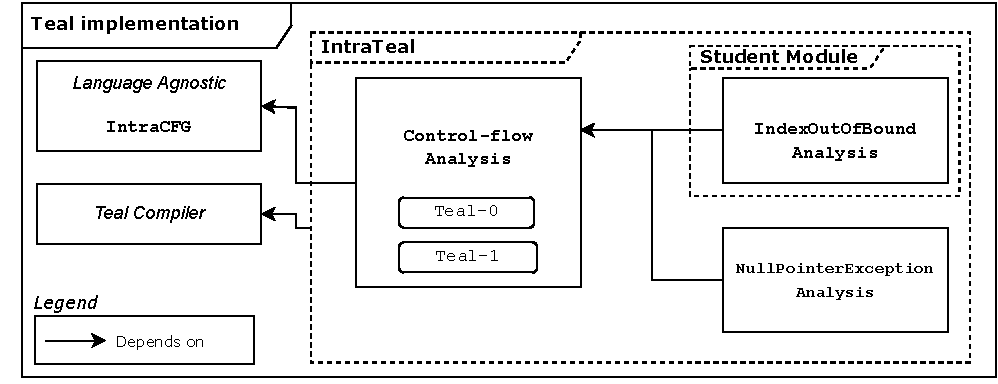
\includegraphics[scale=0.65]{kappa/img/architectureteal.pdf}
    \caption{\label{fig:IntraTeal} Overall architecture of \textsc{IntraCFG} instantiated for the Teal language.}
\end{figure}

% The Teal programming language is used for teaching purposes
% and provides a simple and easy-to-learn syntax for students to understand the
% concepts of static program analysis (see Section~\ref{sec:teal}).
As part of the course, the complete source code of \textsc{IntraTeal} was provided 
to students, along with instructions and guidelines for utilizing the API to implement 
their analyses. We also made available a reference implementation of the \code{NullPointerException} 
analysis. To extend their understanding and skills, we then asked students to implement 
an \code{IndexOutOfBound} analysis on the interval abstract domain. This exercise allowed the 
students to apply the concepts they had learned in a practical setting and gain a 
deeper understanding of dataflow analysis.

Another key aspect of \textsc{IntraTeal} and \textsc{IntraJ} implementations is that they
construct enhanced control sensitive CFGs, i.e., it understands that the following code, 
dereferencing \code{x} inside the body of the if-statement, is safe:
\begin{lstlisting}[language=JastAdd]
if (x != null){
  x.f = 1
}
\end{lstlisting}
Control sensitive CFGs are a more precise representation of the control flow of a program, as they take
into account the different behavior when a branching condition is true or false. This is achieved by
using HOAs to synthesise two AST nodes, i.e., \astnode{ControlTrue} and \astnode{ControlFalse}, for each
comparison operator, e.g.,  ``$\le$'', ``$==$'', ``$!=$'', inside a conditional expression.
These HOAs are used to enhance the control flow of the program with the information that can be inferred from
it. 
\begin{figure}
	\centering
	\begin{tikzpicture}
		\node (a) at (0,0) {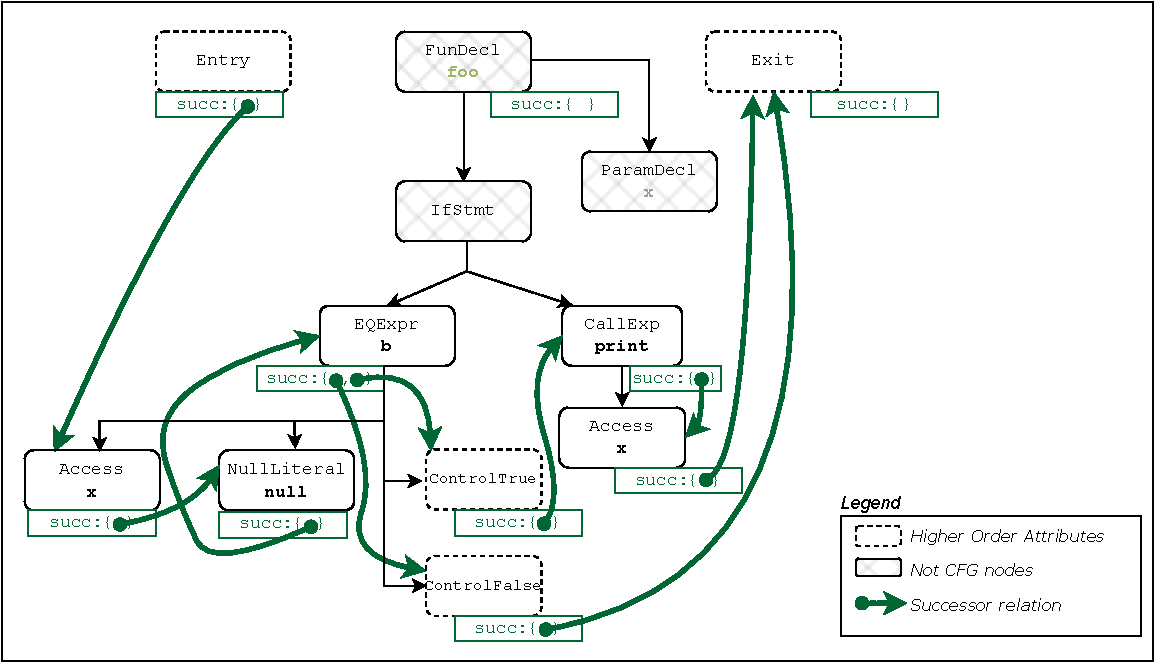
\includegraphics[scale=0.55]{kappa/img/TEALExample.pdf}};
		\node[scale=0.7] (b) at (3.5,0.45) {
			\begin{lstlisting}[language=JastAdd]
fun foo(x) = {
  if(x==null){
    print(x);
  }
}
			\end{lstlisting}
		};
	\end{tikzpicture}
	\caption{\label{fig:ExampleTEAL} Example of control sensitivity in \textsc{IntraTeal}.}
\end{figure}
\begin{lstlisting}[language=JastAdd,label={lst:ControlTrueEq}, caption={Transfer function for \astnode{ControlTrue} HOA.}]
eq ControlTrue.nullnessTransfer(NullDomain lattice) = new NullDomain(lattice).join(getCond().getImplicitAssignment());
\end{lstlisting}
Figure~\ref{fig:ExampleTEAL} shows \textsc{IntraTeal}'s control sensitive CFG for a simple 
program with an if-statement. The \astnode{ControlTrue} and \astnode{ControlFalse} HOAs are
used to distinguish the execution path when the condition in the if-statement evaluates to 
true or false, respectively. The \code{NullPointerException} analysis can benefit from this more refined CFG.
In Listing~\ref{lst:ControlTrueEq}, we show how this enhanced CFG is used to improve the precision of the analysis.
The Listing shows the equation for the transfer function of the \astnode{ControlTrue} HOA.
Specifically, the transfer function for the \astnode{ControlTrue} HOA
records the effect of the implicit assignment\footnote{Modelled as assertions in~\cite{spa}} when the condition of the \astnode{IfStmt} evaluates to true.
In this case, the variable \texttt{x} is assigned the value \texttt{null} and the \astnode{ControlTrue}'s transfer function
records this information.

\begin{minipage}{0.45\textwidth}
  \begin{lstlisting}[language=JastAdd,caption={Control sensitivity to improve null pointer analysis.}, label={lst:control-null}]
if(x!=null){
//x is not null here
}
  \end{lstlisting}
  \end{minipage}\hfill%
  \begin{minipage}{0.45\textwidth}
  \begin{lstlisting}[language=JastAdd,caption={Control sensitivity to improve interval analysis.}, label={lst:control-interval}]
if(x > 4 and x <= 6){
  //x is [5,6] here
}
  \end{lstlisting}
\end{minipage}\\
For the example in Listing~\ref{lst:control-null} the \astnode{ControlTrue} and \astnode{ControlFalse}
HOAs are used to keep track of the information that the object \texttt{x} is not null
in the \emph{then} branch and null in the \emph{else} branch.
This information is used to improve the precision of the analysis and provide
more accurate results without affecting the performance of the analysis.

We also asked students to use the \astnode{ControlTrue} and \astnode{ControlFalse}
HOAs to improve the precision of the interval analysis. Similarly to the previous example, in 
Listing~\ref{lst:control-interval} the \astnode{ControlTrue} and \astnode{ControlFalse}
are used to keep track of the information that the object \texttt{x} is in the interval $[5,6]$.


The task assigned to the students was to implement an \texttt{IndexOutOfBound} analysis on the interval domain.
The interval domain, being an infinite domain, poses a significant challenge for
dataflow analysis. In particular,
the iterative nature of dataflow analysis algorithms, which rely on the computation
of a sequence of approximations, may not terminate when applied to an infinite domain.
Even if the computation terminates, it can result in an excessive consumption of computational resources. 
The example in Figure~\ref{fig:nonConverging}
illustrates a non-converging program.
\begin{figure}
	\centering
	\begin{tikzpicture}
		\node (a) at (3.5,0) {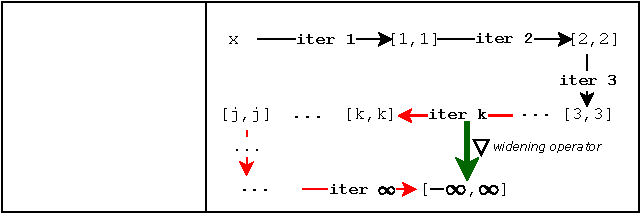
\includegraphics[scale=1]{kappa/img/non-convergin.pdf}};
		\node[scale=1] (b) at (-0.2,0) {
			\begin{lstlisting}[language=JastAdd]
fun foo(x) = {
  x := 0;
  while (true) {
    x = x + 1;
  }
}
			\end{lstlisting}
		};
	\end{tikzpicture}
	\caption{\label{fig:nonConverging} Trivial example of non-converging analysis.
  The {\color{red}red} path represents the non-converging evaluation sequence.
  The analysis keeps changing the value of the variable \code{x} without ever
  reaching a fix-point. The {\color{ForestGreen}green} path represents a
  sequence converging to a fix-point by using the widening operator.
  }
\end{figure}

To ensure the termination of the analysis, the students were required to
define their own widening operator~\cite{Bagnara2003Widening}.
However, \textsc{JastAdd} circular attributes, which are used to implement dataflow
analysis, do not natively support widening operators, as they are designed
to work only on finite lattices. To overcome this limitation, an ad-hoc solution
solution was implemented to trigger the widening operator after a certain
number of steps.

This experience highlights the need for native support for widening and narrowing
operators in \textsc{JastAdd}, to allow static analysis developers to effectively deal with
infinite lattices. In the future, we plan to investigate the implementation of this
feature in \textsc{JastAdd} to facilitate the development of static analysis tools.


\section{IDE Integration}
\label{sec:IDEIntegration}
In this Section, we focus on the integration of \textsc{IntraJ} and \textsc{IntraTeal} with different
IDEs and developer tools. We first describe the integration of \textsc{IntraJ} with
IDEs that support the Language Server Protocol (LSP)~\cite{lsp}, such as
\textsc{Visual Studio Code}~\cite{vscode}, \textsc{Emacs}~\cite{emacs}, and \textsc{Vim}\cite{vim}, using
the MagpieBridge~\cite{luo_et_al:LIPIcs:2019:10813} framework. We then describe the
integration of \textsc{IntraJ} and \textsc{IntraTeal} with \textsc{CodeProber}~\cite{risberg2022property},
a tool for visualising and exploring the results of compilers and static analysis tools.
Our work on integrating \textsc{IntraJ} with different IDEs via the \textsc{MagpieBridge}
framework has gained attention from the \textsc{MagpieBridge} maintainer and resulted in an invitation
to present at the \textsc{PRIDE}\footnote{\textbf{P}ractical \textbf{R}esearch \textbf{IDE}s.} workshop, held in conjunction with \textsc{ECOOP 2022}, with the
title \emph{``Source-Level Dataflow-Based Fixes: Experiences From Using \textsc{IntraJ} and \textsc{MagpieBridge}''}.

This integration process and evaluation are not covered in any of the papers included in this thesis.
However, it was developed as an application of the research and methods previously
described in these papers, and was carried out subsequently.

\subsubsection{LSP support via MagpieBridge: warnings, quick-fixes and bug explanations}
\begin{figure}
  \centering
  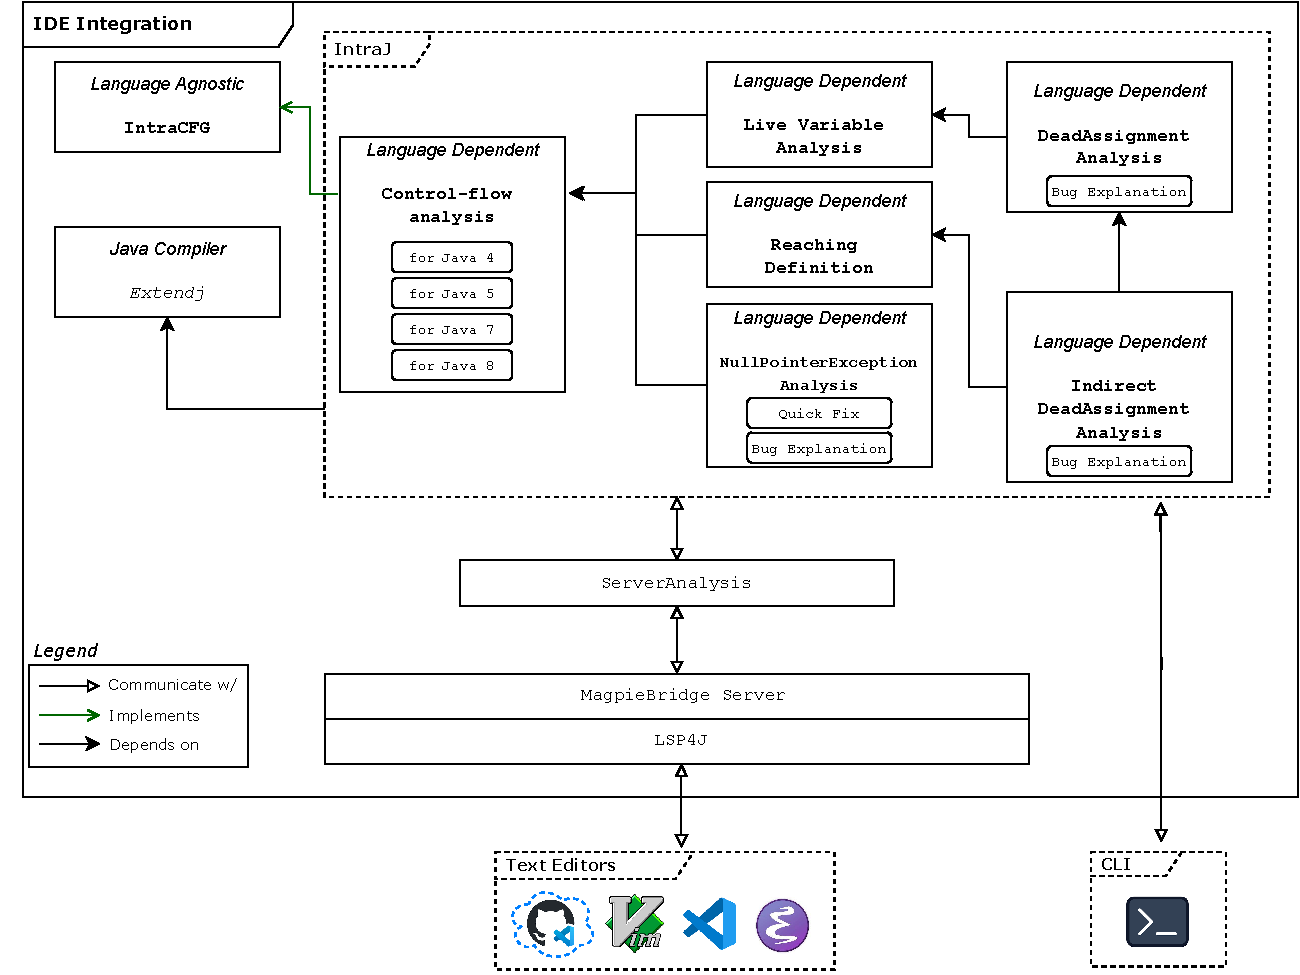
\includegraphics[width=0.92\textwidth]{kappa/img/IDEIntegration.pdf}
  \caption{\label{fig:IDEIntegration} Integration of \textsc{IntraJ} with IDEs through the use of the \textsc{MagpieBridge} framework.}
\end{figure}
Initially, \textsc{IntraJ} was developed as a command-line tool, which performance was competitive
compared to existing industrial tools. However, we recognized the potential
for further improvement, by exploiting the on-demand evaluation feature of \textsc{JastAdd}.
On-demand evaluation enables the execution of dataflow analyses
on methods within open files, as opposed to the entire codebase. This approach
allows for local and in real-time feedback on complex bugs, providing developers
with instantaneous insights, facilitating the debugging process.
To achieve this, we used the \textsc{MagpieBridge} framework, which facilitates the integration
of static analysers with IDEs that support the LSP. \textsc{MagpieBridge} provides an
abstraction layer between the IDE and the static analysis tool, simplifying the
integration process and allowing for the development of IDE plug-ins with minimal effort.
\textsc{MagpieBridge} provides an abstraction layer between the IDE and the static
analysis tool allowing the display of warnings, quick-fixes, and explanations
for bugs within the IDE, providing developers with an immediate and convenient way to
access and interact with analysis results, while also facilitating communication
between the static analysis tool and the IDE. Additionally, the framework allows
for the display of web pages within the IDE, providing developers with a new level
of support for visualization, customizable user interfaces, and a better way to
interact with analysis results.

Figure~\ref{fig:IDEIntegration} illustrates the integration of \textsc{IntraJ} with
different IDEs. \textsc{ServerAnalysis} is a component that we developed to handle the
communication between \textsc{IntraJ} and the \textsc{MagpieBridge} Server. It is responsible
for maintaining a record of the active analyses and forwarding events in the editor,
such as the save command or opening of a file, to \textsc{IntraJ}.
The results of the analysis are then sent back to the \textsc{MagpieBridge}, which subsequently
forwards them to the editor, displaying warnings, quick-fixes, and explanations
to the developer.
\begin{figure}[ht]
  \centering
  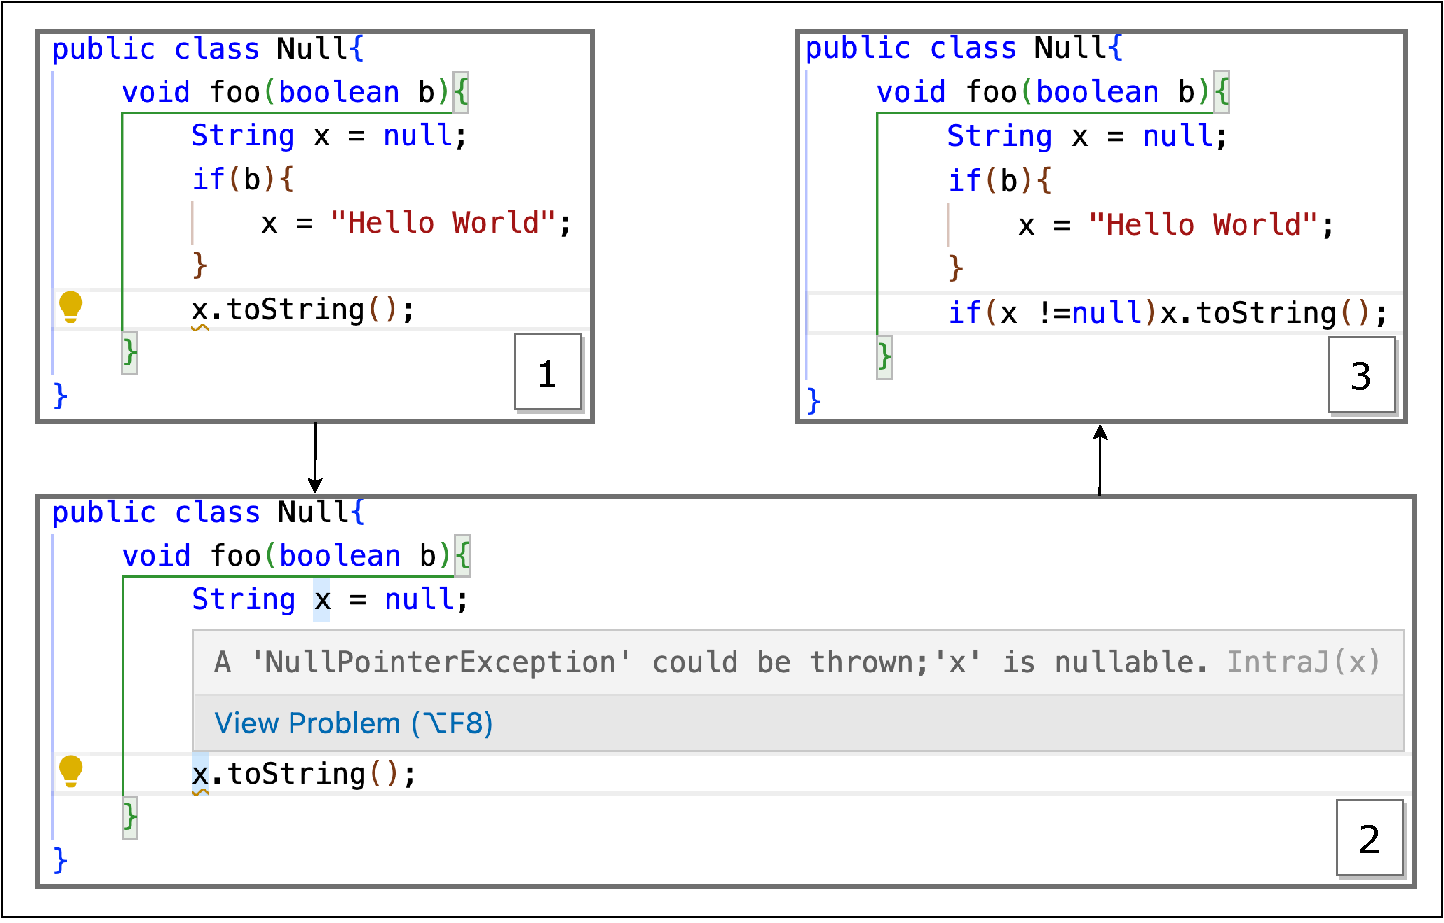
\includegraphics[width=0.92\textwidth]{kappa/img/IDEExample.pdf}
  \caption{\label{fig:IDEExample} Bug detection and quick-fix in \textsc{Visual Studio Code} using \textsc{IntraJ}.
  1. The \texttt{NullPointerException} is detected by \textsc{IntraJ} (squiggly line under \code{x}) with a quick-fix available (
\includegraphics[height=8pt]{kappa/img/bulb.png}).
  2. The user can hover over the warning to see an explanation of the issue.
  3. The user can click on the quick-fix icon (
\includegraphics[height=8pt]{kappa/img/bulb.png}) to apply the fix.
  }
\end{figure}
To enable a better user experience, we extended the functionality of the existing analysis.
Specifically, we enhanced the \texttt{NullPointerException} analysis to not only detect issues
but also provide developers with quick fixes and explanations, allowing them to address
the problems more efficiently. Additionally, we enhanced the \texttt{(Indirect) Dead Assignment} analysis
to provide explanations, giving developers a deeper understanding of the issues detected.
Figure~\ref{fig:IDEExample} illustrates an example of interaction between \textsc{IntraJ} and
\textsc{Visual Studio Code}. More specifically, illustrates an instance of a \texttt{NullPointerException}
detected by \textsc{IntraJ} and its representation within the IDE.
The ``
\includegraphics[height=8pt]{kappa/img/bulb.png}''  icon indicates that an quick-fix is available,
which can be applied by clicking on the icon.

\subsubsection{Visualisation via \textsc{CodeProber}}
In this Section, we will give an overview of the integration of \textsc{IntraTeal}
with \textsc{CodeProber}, a tool for visualizing and
exploring the results of compilers and static analysers. \textsc{CodeProber}
allows developers to interact with the results of the analysis in a visual and intuitive
manner. It enables real-time interaction with the AST node's attributes and the source code,
enabling analysis developers to explore results and partial results, making
debugging and troubleshooting more efficient with respect the traditional debugging
approaches. As a browser-based tool that is not restricted to the Language Server Protocol,
\textsc{CodeProber} enables the visualisation of analysis results in different
formats, including, but not limited to, graph representation and other visual forms, beyond
simply displaying warnings.
\begin{figure}[H]
  \centering
  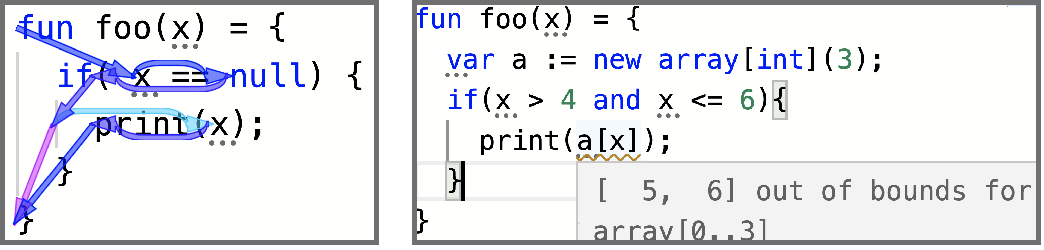
\includegraphics[width=0.92\textwidth]{kappa/img/CP.pdf}
  \caption{\label{fig:CodeProber} Interaction of \textsc{IntraTeal} in \textsc{CodeProber}.}
\end{figure}
The example in Figure~\ref{fig:CodeProber} shows the visual representation of the CFG on
top of the source code. The CFG is generated by \textsc{IntraTeal} and visualized by
\textsc{CodeProber}. The graph is rendered automatically at each change in the source code,
allowing developers to understand the flow of the program and all the possible execution paths of the
analysis in real-time.

We used the \textsc{IntraTeal} and \textsc{CodeProber} integration in the Program analysis
course. Students were able to understand the CFG and the flow of the program and
were asked to identify \textsc{IndexOutOfBound} exceptions. Students were able to
observe their progress and the outcomes of their analysis within a realistic IDE.



\section{\textsc{JFeature}: Java Feature Extractor}
\label{sec:JFeature}
\textsc{JFeature} is a RAG-based static analysis tool for the Java programming language that extracts
syntactic and semantic features from Java programs. The tool is designed to assist
researchers and developers in selecting appropriate software corpora to better evaluate the robustness
and performance of software tools, such as static analysers.
\textsc{JFeature} is implemented as an extension of the \textsc{ExtendJ} Java compiler. It is declarative
and extensible, allowing for the easy addition of new queries. In this Section, 
we give an overview of this work, and more details are available in Paper~\ref{paper:jfeature}.

The need for \textsc{JFeature} arose during the evaluation of \textsc{IntraJ}.
While analysing Java projects from the \textsc{DaCapo Benchmark suite}~\cite{DaCapo:paper} corpus to evaluate the precision
of \textsc{IntraJ} on Java 8 projects, it became apparent that there were no Java 8 projects
in the \textsc{Da Capo Benchmark suite}. Further investigation revealed that many
commonly used software corpora in the field of static analysis were lacking
representation of Java 8 projects.

To address this problem, we developed \textsc{JFeature}, a tool that extracts features from
Java programs categorised by the Java version they were introduced in.
The goal of \textsc{JFeature} is to provide insight and an overview of
the composition of a Java project or corpus, specifically in terms of the different
Java features categorized by the Java version in use.
\textsc{JFeature} comes with twenty-six predefined queries and can be easily extended
with new ones. Since \textsc{JFeature} is built on top of the \textsc{ExtendJ} compiler, \textsc{JFeature} has access
to all the information computed by the compiler, allowing the definition of complex
queries.
In Figure~\ref{fig:JFeature}, we show the architecture of \textsc{JFeature}.
\begin{figure}[H]
  \centering
  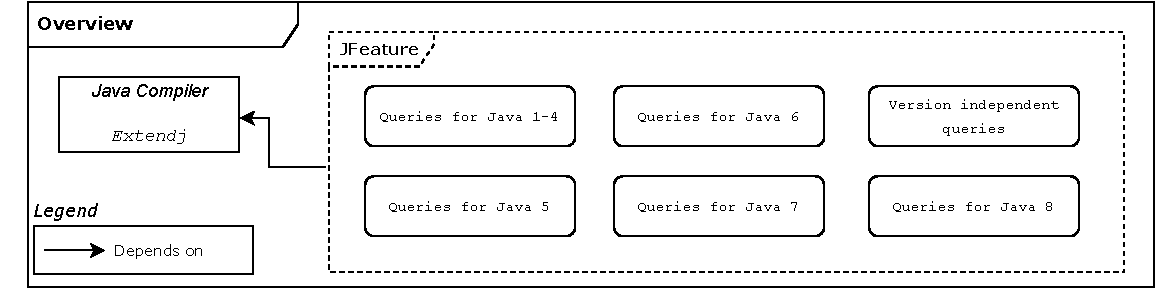
\includegraphics[width=1\textwidth]{kappa/img/JFeature.pdf}
  \caption{\label{fig:JFeature} \textsc{JFeature} architecture.}
\end{figure}

We conducted a case study, applying \textsc{JFeature} to four widely used corpora in the
program analysis area: the \textsc{Da Capo Benchmark suite}~\cite{DaCapo:paper}, \textsc{Defects4J}~\cite{just2014defects4j},
\textsc{Qualitas Corpus}~\cite{QualitasCorpus:APSEC:2010}, and \textsc{XCorpus}~\cite{dietrich2017xcorpus}.
The results showed that Java 1-5 features were predominant among the corpora,
suggesting that some of the corpora may be less suited for the evaluation of
tools that address features in Java 7 and 8.
In addition to evaluating corpora, we showed how \textsc{JFeature} could also be used for other
applications such as longitudinal studies of individual Java projects and the creation
of new corpora. In Paper~\ref{paper:jfeature}, we also demonstrate a practical application of how \textsc{JFeature} can
be extended to capture more complex semantic features by writing queries using the RAGs formalism.


